%Contents of the plugin features section of D5.5
In order to guide the user on how best to exploit certain features of the MPI Parameters Plugin we will focus on the the Fish School Simulator application (FSSIM) \cite{Mostaccio05}.

\subsubsection{Multiple MPI flavors}\label{para:MPI-mult}

The MPI Parameters plugin offers some degree of support for three different implementations of  MPI: IBM MPI, Intel MPI and OpenMPI. In these cases, the keywords {\tt ibm}, {\tt intel}, or {\tt openmpi} should appear at the beginning of the configuration file.  Then, the plugin interprets that the user is specifying command line options and modifies the application execution command accordingly to the syntax established by the specific implementation.

Assuming that the user has included the parameter for tuning the eager limit in the configuration file, the MPI Parameters plugin will, for example, generate the following command line in each case:

\begin {itemize}
\item IBM MPI: mpiexec -n 64 executable -eager\_limit 16384
\item Intel MPI: mpiexec -genv I\_MPI\_EAGER\_THRESHOLD 16384 -n 64 executable
\item OpenMPI: mpiexec -mca osc\_pt2pt\_eager\_limit 16384 -n 64 executable
\end{itemize}

In any other case, the plugin interprets that the parameters indicated by the user are environment variables and produces the corresponding export commands before re-executing the application.  In addition, three example configuration files are provided along with the MPI Parameters plugin, one for each supported implementation (Intel MPI, IBM MPI and OpenMPI). They can be used as a quite complete starting point for tuning a rich set of MPI parameters. However, the user can also modify them (eliminating, adding or changing parameters) with the objective of fitting them to a particular application.

The three configuration files included with the PTF release are the following:

\begin {enumerate}
\item IBM MPI

\begin{verbatim}
MPIPO_BEGIN ibm
eager_limit=4096:2048:65560;
buffer_mem=8388608:2097152:134217728;
use_bulk_xfer=yes,no;
bulk_min_msg_size=4096:4096:1048576;
pe_affinity=yes,no;
cc_scratch_buf=yes,no;
wait_mode=nopoll,poll;
css_interrupt=yes,no;
polling_interval=100000:10000:1000000;
SEARCH=gde3;
MPIPO_END
\end{verbatim}

\item Intel MPI

\begin{verbatim}
MPIPO_BEGIN intel
I_MPI_EAGER_THRESHOLD=4096:2048:65560;
I_MPI_INTRANODE_EAGER_THRESHOLD=4096:2048:65560;
I_MPI_SHM_LMT=shm,direct,no;
I_MPI_SPIN_COUNT=1:2:500;
I_MPI_SCALABLE_OPTIMIZATION=yes,no;
I_MPI_WAIT_MODE=yes,no;
I_MPI_USE_DYNAMIC_CONNECTIONS=yes,no;
I_MPI_SHM_FBOX=yes,no;
I_MPI_SHM_FBOX_SIZE=2048:512:65472;
I_MPI_SHM_CELL_NUM=64:4:256;
I_MPI_SHM_CELL_SIZE=2048:1024:65472;
SEARCH=gde3;
MPIPO_END
\end{verbatim}

\item OpenMPI

\begin{verbatim}
MPIPO_BEGIN openmpi
mpi_paffinity_alone=0,1;
btl_openib_eager_limit=1024:2048:65560;
btl_openib_free_list_num=2:4:128;
btl_openib_use_eager_rdma=0,1;
btl_openib_eager_rdma_num=1:2:32;
btl_sm_eager_limit=1024:2048:65560;
btl_sm_num_fifos=1:1:10;
btl_sm_fifo_size=2048:512:65472;
btl_sm_free_list_num=2:4:128;
MPIPO_END
\end{verbatim}
\end {enumerate}

\subsubsection{Genetic search}\label{para:MPI-gen}

PTF has been enriched with the implementation of a search strategy based on the \textit{Generalized Differential Evolution 3 (GDE3)} genetic algorithm. In this strategy a population of ten initial scenarios is randomly generated and executed, then, an iterative process is followed, generating new populations by selecting the best five scenarios (those with the smallest execution time) for the next generation (elitism), generating five new scenarios by crossing over the previous population (crossover), and introducing mutations with a fixed probability (mutation). The number of iterations can be configured, but, generally, a close to optimal solution can be found in less than 30 iterations (generations).

For our use cases we have used a medium size population of fishes (64K), to avoid long executions, and have run the MPI application on 64 compute cores. In addition, given that it is not possible to test a large set of parameters combinations exhaustively in a reasonable time, we have used the exhaustive search strategy for a very limited configuration (see Table \ref{table:MPIConfigFileExhaustive}) of the parameters, and the heuristic search strategy for a more complete configuration (see Table \ref{table:MPIConfigFileGDE3}).

\begin{table}[tb]
	\centering
	\begin{footnotesize}
		\begin{tabular}{| l | }
		\hline
			\\
			MPI\_PIPO BEGIN ibm \\
			eager\_limit=4096:15366:65560; \\
			use\_bulk\_xfer=yes,no; \\
			bulk\_min\_msg\_size=4096:4096:1048576; \\
			task\_affinity=CORE,MCM; \\
			pe\_affinity=yes,no; \\
			cc\_scratch\_buf=yes,no; \\
			MPI\_PIPO END \\
			\\
		\hline
		\end{tabular}
	\caption{Configuration file for the exhaustive search.}
	\label{table:MPIConfigFileExhaustive}
	\end{footnotesize}
\end{table}


\begin{table}[tb]
	\centering
	\begin{footnotesize}
		\begin{tabular}{| l | }
		\hline
			\\
			MPIPO\_BEGIN ibm\\
			eager\_limit=4096:2048:65560;\\
			buffer\_mem=8388608:2097152:134217728;\\
			use\_bulk\_xfer=yes,no;\\
			bulk\_min\_msg\_size=4096:4096:1048576;\\
			cc\_scratch\_buf=yes,no;\\
			wait\_mode=nopoll,poll;\\
			css\_interrupt=yes,no;\\
			polling\_interval=100000:10000:1000000;\\
			task\_affinity=CORE,MCM; \\
			pe\_affinity=yes,no; \\
			SEARCH=gde3; \\
			MPI\_PIPO END \\
			\\
		\hline
		\end{tabular}
	\caption{Configuration file for the GDE3 search.}
	\label{table:MPIConfigFileGDE3}
	\end{footnotesize}
\end{table}


The exhaustive search strategy generates all possible combinations of the selected parameters and values, 320 in our example. Each scenario is executed and the one with the smallest wall time is chosen as the best one. The best combination corresponds to scenario 217: {\tt use\_bulk\_xfer} yes, {\tt bulk\_min\_msg\_size} 796672, {\tt cc\_scratch\_buf} no, {\tt task\_affinity} CORE, {\tt eager\_limit} 50194, {\tt pe\_affinity} yes. The execution time for this scenario was 2.8 sec, which is 1.6 times better than the time for the execution using the parameters default values (4.4 sec). The drawback is that for finding the optimal scenario in the set of tested ones, PTF needed 21505.2 sec (almost 6 hours) for the use case here.

The genetic search strategy (GDE3) can also be used for the same tuning space, but can even handle much larger tuning spaces consisting of significantly more parameters and possible values. For the use case we provide here, it executes 20 different scenarios in 1138.65 sec (approximately 20 min), which reduces the analysis time by a factor of 19 with respect to the exhaustive search. The best scenario in this case was found to be number 14: {\tt use\_bulk\_xfer} no, {\tt bulk\_min\_msg\_size} 988789, {\tt css\_interrupt} no, {\tt wait\_mode} poll, {\tt polling\_interval} 636027, {\tt cc\_scratch\_buf} no, {\tt task\_affinity} CORE, {\tt buffer\_mem} 102205313, {\tt eager\_limit} 59434, {\tt pe\_affinity} yes. The execution time for this scenario was 2.8 sec, again significantly better than the one obtained with the default values and now the search time has also been significantly reduced.  These results demonstrate that using the genetic search strategy can lead to results that are almost as good as the ones produced by the exhaustive search in only a fraction of the time needed for the latter.

\subsubsection{Eager-limit parameter strategy}\label{para:MPI-gen}

The MPI Parameters plugin includes an automatic strategy for determining if it is worthy to include the eager limit and memory buffer parameters into the plugin search space. Moreover, if it determines that it is worthy to include these parameters in the search, it will automatically generate the range of values that should be searched, trying to shrink this range in order to reduce the size of the search space. For using this strategy, the user only has to specify in the configuration file the option {\tt AUTO\_EAGER\_LIMIT=<eager-limit parameter>,<buffer-mem parameter>}. In our case, using IBM MPI, the configuration option is {\tt AUTO\_EAGER\_LIMIT=eager\_limit, buffer\_mem;}.

Here we test the plugin using this configuration option, where the FSSIM application was executed with a medium size population of 64K fishes and on 64 cores. The plugin determines that it is worthy to include the {\tt eager\_limit} and {\tt buffer\_mem} parameters into the search space because the total number of bytes communicated in point-to-point messages smaller than 64Kb was found to be greater than 30\% of the total number of bytes communicated in point-to-point messages. In addition, the plugin determines that the search range for the eager limit parameter should be between 1Kb and 32Kb because more than 80\% of the messages sent eagerly were in this range. Finally, the plugin uses the values determined for the eager limit and expression \ref{eqn:mem_buff} to compute the range for the buffer mem parameter range (128Kb to 4Mb).

\begin{equation}
	mem\_buff = 2{n}*{max(eager\_limit,64)}
\label{eqn:mem_buff}
\end{equation}

\begin{figure}[bth]
  \center
  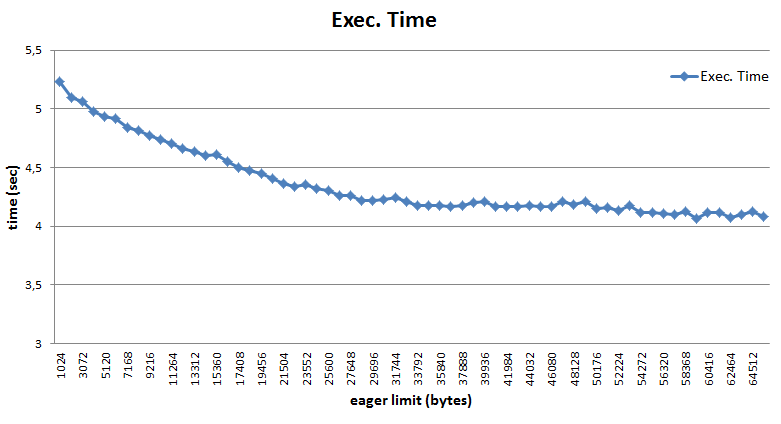
\includegraphics[width=0.65\paperwidth]{../BPG/images/MPIFssimEager.png}
	\caption{FSSIM execution time for different values of the eager limit and memory buffer parameters (IBM MPI).}
	\label{fig:fssimEager}
\end{figure}

\begin{figure}[bth]
  \center
  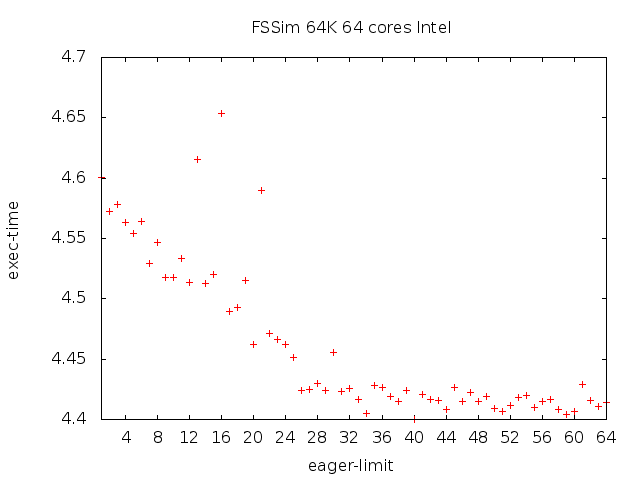
\includegraphics[width=0.65\paperwidth]{../BPG/images/MPImanual64cpu64kf.png}
	\caption{FSSIM execution time for different values of the eager limit and memory buffers parameters (Intel MPI).}
	\label{fig:fssimEagerIntel}
\end{figure}

Figures \ref{fig:fssimEager} and \ref{fig:fssimEagerIntel} clearly show that increasing the eager limit for this application up to approximately 30Kb produces  significant performance improvements, and that beyond this size no extra gains are obtained. This demonstrates that the eager limit strategy is successfully identifying the range of values that should be explored by the user for finding the best value for this parameter.

